\section{Results}
\label{sec:results}

Unless stated otherwise, results are for leave-one-year-out evaluation at $L=3$\,h, and every
LightGBM variant is a five-seed ensemble (Section~\ref{sec:methods}). The pooled 24\,h test set
has \pv{ens24.n} station-hours and \pv{ens24.events} event hours.

\subsection{Baselines and model families}

\begin{table}[t]
\centering
\small
\begin{tabular}{lcccccccc}
\toprule
 & \multicolumn{4}{c}{$h=24$\,h} & \multicolumn{4}{c}{$h=6$\,h} \\
\cmidrule(lr){2-5}\cmidrule(lr){6-9}
Model & AP & AUC & BSS & hit@2\% & AP & AUC & BSS & hit@2\% \\
\midrule
Persistence & \pv{ens24.AP.persistence} & \pv{ens24.AUC.persistence} & \pv{ens24.BSS.persistence} & \pv{ens24.hit.persistence}
            & \pv{ens6.AP.persistence} & \pv{ens6.AUC.persistence} & \pv{ens6.BSS.persistence} & \pv{ens6.hit.persistence} \\
Climatology & \pv{ens24.AP.climatology} & \pv{ens24.AUC.climatology} & \pv{ens24.BSS.climatology} & \pv{ens24.hit.climatology}
            & \pv{ens6.AP.climatology} & \pv{ens6.AUC.climatology} & \pv{ens6.BSS.climatology} & \pv{ens6.hit.climatology} \\
\midrule
GBM C       & \pv{ens24.AP.C} & \pv{ens24.AUC.C} & \pv{ens24.BSS.C} & \pv{ens24.hit.C}
            & \pv{ens6.AP.C} & \pv{ens6.AUC.C} & \pv{ens6.BSS.C} & \pv{ens6.hit.C} \\
GBM D       & \pv{ens24.AP.D} & \pv{ens24.AUC.D} & \pv{ens24.BSS.D} & \pv{ens24.hit.D}
            & \pv{ens6.AP.D} & \pv{ens6.AUC.D} & \pv{ens6.BSS.D} & \pv{ens6.hit.D} \\
GBM D0      & \pv{ens24.AP.D0} & \pv{ens24.AUC.D0} & \pv{ens24.BSS.D0} & \pv{ens24.hit.D0}
            & \pv{ens6.AP.D0} & \pv{ens6.AUC.D0} & \pv{ens6.BSS.D0} & \pv{ens6.hit.D0} \\
GBM E       & \pv{ens24.AP.E} & \pv{ens24.AUC.E} & \pv{ens24.BSS.E} & \pv{ens24.hit.E}
            & \pv{ens6.AP.E} & \pv{ens6.AUC.E} & \pv{ens6.BSS.E} & \pv{ens6.hit.E} \\
GBM Rshift  & \pv{ens24.AP.Rshift} & \pv{ens24.AUC.Rshift} & \pv{ens24.BSS.Rshift} & \pv{ens24.hit.Rshift}
            & \pv{ens6.AP.Rshift} & \pv{ens6.AUC.Rshift} & \pv{ens6.BSS.Rshift} & \pv{ens6.hit.Rshift} \\
GBM Rperm1  & \pv{ens24.AP.Rperm1} & \pv{ens24.AUC.Rperm1} & \pv{ens24.BSS.Rperm1} & \pv{ens24.hit.Rperm1}
            & \pv{ens6.AP.Rperm1} & \pv{ens6.AUC.Rperm1} & \pv{ens6.BSS.Rperm1} & \pv{ens6.hit.Rperm1} \\
GBM D0m     & \pv{ens24.AP.D0m} & \pv{ens24.AUC.D0m} & \pv{ens24.BSS.D0m} & \pv{ens24.hit.D0m}
            & \pv{ens6.AP.D0m} & \pv{ens6.AUC.D0m} & \pv{ens6.BSS.D0m} & \pv{ens6.hit.D0m} \\
GBM D0cat   & \pv{ens24.AP.D0cat} & \pv{ens24.AUC.D0cat} & \pv{ens24.BSS.D0cat} & \pv{ens24.hit.D0cat}
            & \pv{ens6.AP.D0cat} & \pv{ens6.AUC.D0cat} & \pv{ens6.BSS.D0cat} & \pv{ens6.hit.D0cat} \\
GBM Ecat    & \pv{ens24.AP.Ecat} & \pv{ens24.AUC.Ecat} & \pv{ens24.BSS.Ecat} & \pv{ens24.hit.Ecat}
            & \pv{ens6.AP.Ecat} & \pv{ens6.AUC.Ecat} & \pv{ens6.BSS.Ecat} & \pv{ens6.hit.Ecat} \\
\midrule
Logit C     & \pv{ens24.AP.lgC} & \pv{ens24.AUC.lgC} & \pv{ens24.BSS.lgC} & \pv{ens24.hit.lgC}
            & \pv{ens6.AP.lgC} & \pv{ens6.AUC.lgC} & \pv{ens6.BSS.lgC} & \pv{ens6.hit.lgC} \\
Logit D0    & \pv{ens24.AP.lgD0} & \pv{ens24.AUC.lgD0} & \pv{ens24.BSS.lgD0} & \pv{ens24.hit.lgD0}
            & \pv{ens6.AP.lgD0} & \pv{ens6.AUC.lgD0} & \pv{ens6.BSS.lgD0} & \pv{ens6.hit.lgD0} \\
Logit E     & \pv{ens24.AP.lgE} & \pv{ens24.AUC.lgE} & \pv{ens24.BSS.lgE} & \pv{ens24.hit.lgE}
            & \pv{ens6.AP.lgE} & \pv{ens6.AUC.lgE} & \pv{ens6.BSS.lgE} & \pv{ens6.hit.lgE} \\
\bottomrule
\end{tabular}
\caption{Pooled leave-one-year-out scores ($L=3$\,h). GBM rows are five-seed LightGBM ensembles.
AP: average precision; AUC: ROC-AUC; BSS: Brier skill score against station-month climatology;
hit@2\%: share of event hours (\%) caught when alerting on the top 2\% of hours.}
\label{tab:main}
\end{table}

\begin{figure}[t]
  \centering
  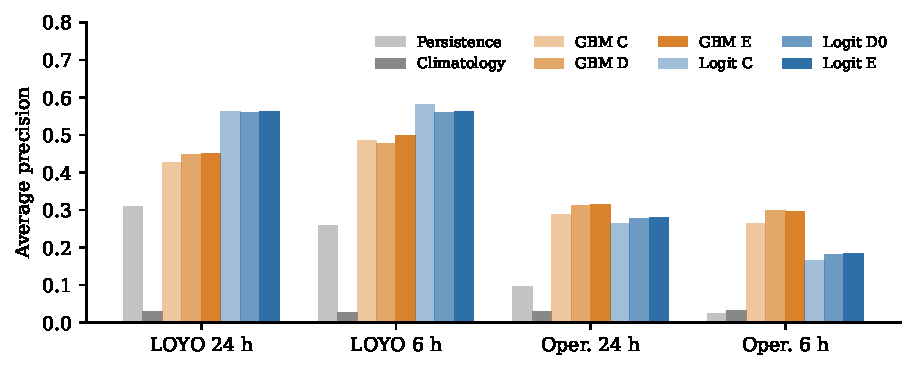
\includegraphics[width=\linewidth]{figures/fig6_models}
  \caption{Average precision by model and evaluation setup ($L=3$\,h). Orange: gradient boosting
  (five-seed ensembles); blue: logistic regression; grey: persistence and climatology.}
  \label{fig:models}
\end{figure}

Table~\ref{tab:main} and Figure~\ref{fig:models} summarise the models. Every learned model is far
above climatology (AP \pv{ens24.AP.climatology}) and persistence (\pv{ens24.AP.persistence}) at
24\,h. Persistence is better at 24\,h than at 6\,h: haze visibility has a strong diurnal cycle, so
the same hour on the next day is a better analogue than six hours later.

The largest differences in the table are between model families, not between feature sets.
Under leave-one-year-out, logistic regression on station state alone reaches AP
\pv{ens24.AP.lgC} at 24\,h, against \pv{ens24.AP.C} for gradient boosting on the same features.
Most of that gap comes from the 2015 fold, the most extreme season, which tree models trained on
milder years cannot extrapolate to. On the operational split the order reverses
(Section~\ref{sec:operational}), so neither family is uniformly better.

\subsection{Single fits cannot resolve the effect (pre-specified analysis)}
\label{sec:seeds}

The protocol specified one LightGBM fit per variant. Under that design, adding the directional
exposure raised pooled 24\,h AP by \pv{loyo24.d.E-D0} \pv{loyo24.ci.E-D0} over D0, which would
have confirmed H1 decisively. The shifted-wind placebo and the missingness control gained almost
as much (Rshift$-$D0 \pv{loyo24.d.Rshift-D0}, D0m$-$D0 \pv{loyo24.d.D0m-D0}). On closer
inspection, nearly all of these pooled differences came from the 2015 fold. There the variants
fell into two groups, with AP near 0.52 or near 0.59, and group membership did not follow feature
content: Ecat, which contains every column of D0cat plus the directional exposure, landed in the
low group while D0cat landed in the high one.

\begin{figure}[t]
  \centering
  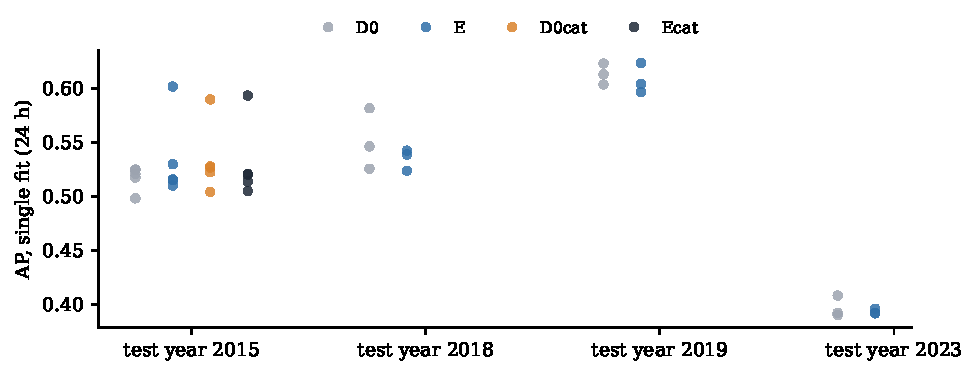
\includegraphics[width=\linewidth]{figures/fig7_seeds}
  \caption{AP of single LightGBM fits that differ only in the random seed (24\,h, $L=3$\,h, one
  test year each). Five seeds for 2015, three for the other years shown.}
  \label{fig:seeds}
\end{figure}

Refitting single folds with different seeds shows why (Figure~\ref{fig:seeds}). In the 2015
fold, D0 ranges from \pv{seed.2015.D0.min} to \pv{seed.2015.D0.max} and E from
\pv{seed.2015.E.min} to \pv{seed.2015.E.max}; the high outcome appears in about one fit in five,
for any variant. Smaller seasons are also affected: in 2018, D0 alone ranges from
\pv{seed.2018.D0.min} to \pv{seed.2018.D0.max}. The seed controls bagging and feature
subsampling, so a single fit is one draw from a wide distribution, and the differences we want to
detect (a few thousandths of AP) are far smaller than its spread. The pre-specified single-fit
comparison is therefore not informative about H1--H3, in either direction. We keep it in
Appendix~\ref{app:extra} and base the conclusions below on five-seed ensembles. Five seeds reduce
but do not remove this noise (for example, Ecat at 6\,h stays an outlier,
Table~\ref{tab:main}, again because of the 2015 fold: \pv{py.6.2015.Ecat} against
\pv{py.6.2015.D0cat} for D0cat), so small single contrasts should be read with that in mind.

\subsection{The directional term with seed ensembles (H1, H3)}

\begin{figure}[t]
  \centering
  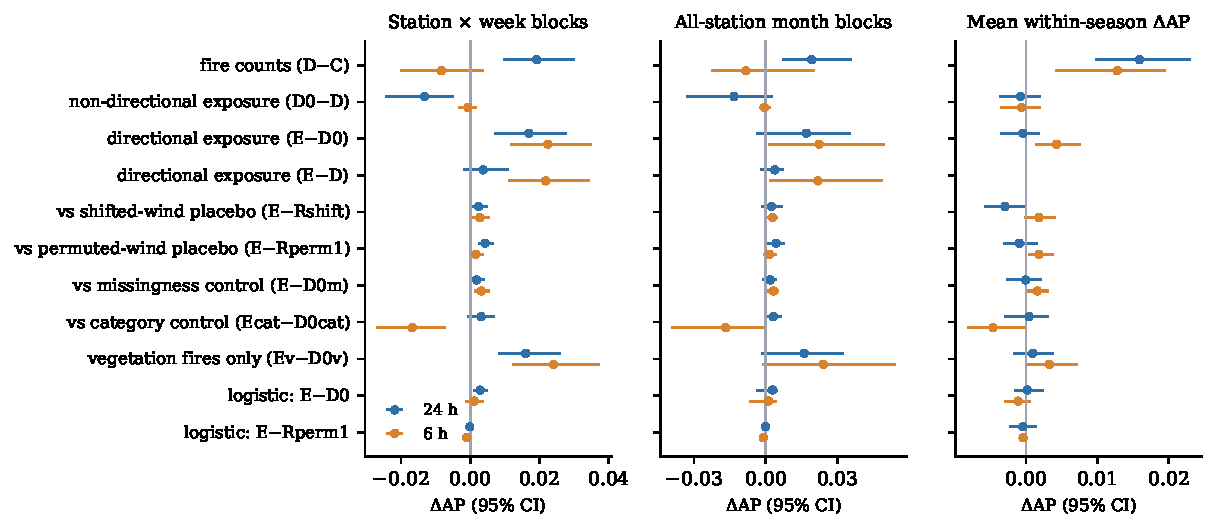
\includegraphics[width=\linewidth]{figures/fig3_ablation}
  \caption{Differences in average precision under leave-one-year-out ($L=3$\,h; LightGBM rows are
  five-seed ensembles), with 95\% block-bootstrap intervals (500 resamples). Left: station
  $\times$ ISO-week blocks. Middle: calendar-month blocks holding all stations together. Right:
  mean of within-year differences over the ten years with at least 100 event hours.}
  \label{fig:ablation}
\end{figure}

With seed ensembles, the directional exposure improves on the matched non-directional model by
\pv{ens24.d.E-D0} \pv{ens24.ci.E-D0} at 24\,h (Figure~\ref{fig:ablation}). Part of that is D0
being low rather than E being high: against the counts-only model, E gains
\pv{erb.24.station-week.E-D} \pv{erb.24.station-week.E-D.ci}. Against the controls, the margin
shrinks to a few thousandths:

\begin{itemize}
  \item placebos: E$-$Rshift \pv{ens24.d.E-Rshift} \pv{ens24.ci.E-Rshift} and E$-$Rperm1
        \pv{ens24.d.E-Rperm1} \pv{ens24.ci.E-Rperm1};
  \item missingness controls: E$-$D0m \pv{ens24.d.E-D0m} \pv{ens24.ci.E-D0m}, and with the
        wind-report categories and category-split exposure already in the model, adding the
        directional exposure changes AP by \pv{ens24.d.Ecat-D0cat} \pv{ens24.ci.Ecat-D0cat}.
\end{itemize}

When each season is weighted equally the picture is the same: E$-$D0 \pv{ens24.sd.E-D0}
\pv{ens24.sci.E-D0}, E$-$Rperm1 \pv{ens24.sd.E-Rperm1} \pv{ens24.sci.E-Rperm1}. Holding all
stations together in calendar-month blocks, which respects the regional extent of haze episodes,
widens the intervals enough that even E$-$D0 includes zero (\pv{erb.24.month.E-D0.ci}; E$-$Rperm1
\pv{erb.24.month.E-Rperm1.ci}).
Year blocks, with only eleven clusters, are coarser still (Appendix~\ref{app:extra}).

The logistic family, which has no seed, agrees: lgE$-$lgD0 \pv{ens24.d.lgE-lgD0}
\pv{ens24.ci.lgE-lgD0} and lgE$-$lgRperm1 \pv{ens24.d.lgE-lgRperm1} \pv{ens24.ci.lgE-lgRperm1}.
At 6\,h the margins are of the same size but somewhat steadier: E is ahead of the missingness
control and the shifted placebo by about 0.003 AP with intervals that exclude zero even with
month blocks (E$-$D0m \pv{erb.6.month.E-D0m} \pv{erb.6.month.E-D0m.ci}; E$-$Rshift
\pv{erb.6.month.E-Rshift} \pv{erb.6.month.E-Rshift.ci}), but not ahead of the permuted placebo
(\pv{erb.6.month.E-Rperm1} \pv{erb.6.month.E-Rperm1.ci}), and the logistic family shows nothing
(lgE$-$lgRperm1 \pv{ens6.d.lgE-lgRperm1} \pv{ens6.ci.lgE-lgRperm1}).

In short, the directional exposure ends up a few thousandths of AP above its controls, and not
consistently. Some station-week intervals exclude zero (E$-$Rperm1 at 24\,h), but the same
contrast is negative or null when seasons are weighted equally, the placebo comparisons change
sign between aggregations (E$-$Rshift per season \pv{ens24.sd.E-Rshift}
\pv{ens24.sci.E-Rshift}), the logistic family shows nothing against the permuted placebo, and the
differences are smaller than the seed noise that remains in five-seed ensembles (Ecat$-$D0cat at
6\,h is \pv{ens6.d.Ecat-D0cat}). The upper ends of the intervals against the placebos and
controls stay below 0.01 AP under every block design. We therefore read any directional
contribution as at most about 0.01 AP, plausibly a few thousandths at 6\,h, and not established
at either horizon. H1, stated against D0 alone, is supported in the pooled score, but
H3 fails: the placebos and non-directional controls reach nearly the same skill, so the gain over
D0 cannot be attributed to direction.

\subsection{Fire counts}

Detection counts improve on station state at 24\,h: D$-$C \pv{ens24.d.D-C} \pv{ens24.ci.D-C}
pooled and \pv{ens24.sd.D-C} \pv{ens24.sci.D-C} per season. With month blocks the pooled interval
is \pv{erb.24.month.D-C.ci}. At 6\,h, where persistence carries most of the signal, the pooled
effect is not distinguishable from zero (\pv{ens6.d.D-C} \pv{ens6.ci.D-C}), although the
per-season mean is positive (\pv{ens6.sd.D-C} \pv{ens6.sci.D-C}). The non-directional exposure adds
nothing on top of the counts when seasons are weighted equally (D0$-$D \pv{ens24.sd.D0-D}
\pv{ens24.sci.D0-D}); pooled, it is slightly worse (\pv{ens24.d.D0-D} \pv{ens24.ci.D0-D}), again
because of the 2015 fold.

\subsection{Where differences arise}

\begin{figure}[t]
  \centering
  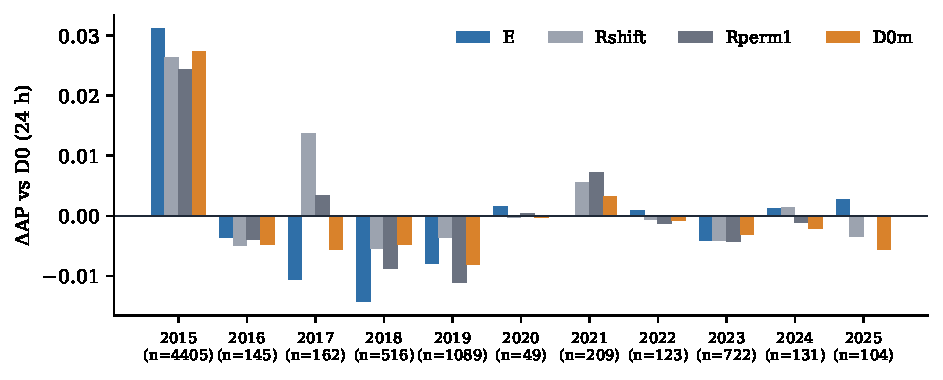
\includegraphics[width=\linewidth]{figures/fig4_years}
  \caption{Within-year change in AP relative to D0 at 24\,h for the directional exposure (E), the
  two placebos and the missingness control, all five-seed ensembles. $n$: event hours.}
  \label{fig:years}
\end{figure}

Figure~\ref{fig:years} splits the 24\,h comparison by test year. The 2015 fold still carries the
largest differences, now of similar size for E and for every control
(\pv{ens24.br.y2015.dE} for E, \pv{ens24.br.y2015.dRshift} for Rshift,
\pv{ens24.br.y2015.dD0m} for D0m), because D0 itself is low in that year
(\pv{py.24.2015.D0}, against \pv{py.24.2015.D} for D and \pv{py.24.2015.C} for C). In the other
two major seasons E is slightly below D0 (2019: \pv{ens24.br.y2019.dE}; 2023:
\pv{ens24.br.y2023.dE}). By reporting convention, E$-$D0 is \pv{ens24.br.ID.dE} at the Indonesian
stations (FU coding) and \pv{ens24.br.MY.dE} at the Malaysian stations (HZ coding).

\subsection{Vegetation fires only}

Removing non-vegetation detections (gas flares, other static sources, offshore platforms) leaves
the conclusions unchanged: D0v scores \pv{ens24.AP.D0v} against \pv{ens24.AP.D0} for D0, and the
directional term adds \pv{ens24.d.Ev-D0v} \pv{ens24.ci.Ev-D0v}, of the same size as with all
detections.

\subsection{Lead time (H2) and latency (H4)}

With no directional contribution detectable at either horizon, H2 (a larger directional gain at
24\,h than at 6\,h) has nothing to compare. For latency, the five-seed ensembles give E$-$D0 at
24\,h of \pv{elat.L0.24.E-D0} with no latency, \pv{elat.L3.24.E-D0} at 3\,h,
\pv{elat.L12.24.E-D0} at 12\,h and \pv{elat.L24.24.E-D0} at 24\,h, and E$-$Rshift of
\pv{elat.L0.24.E-Rshift}, \pv{elat.L3.24.E-Rshift}, \pv{elat.L12.24.E-Rshift} and
\pv{elat.L24.24.E-Rshift} (Figure~\ref{fig:latency}). Both curves are flat: the margin over the
placebo stays within a few thousandths of AP whether the fire data are fresh or a day old, so
there is no directional gain whose decay H4 could describe.

\begin{figure}[t]
  \centering
  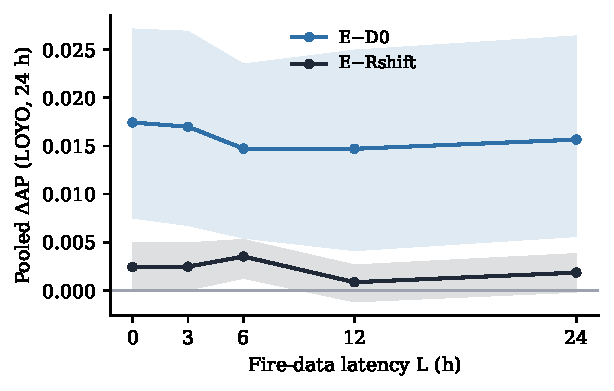
\includegraphics[width=0.62\linewidth]{figures/fig5_latency}
  \caption{Pooled $\Delta$AP at 24\,h under leave-one-year-out as a function of fire-data latency
  $L$ (five-seed ensembles), with 95\% block-bootstrap bands (300 resamples).}
  \label{fig:latency}
\end{figure}

\subsection{Operational split}
\label{sec:operational}

On the deployed configuration (train 2015--2020, test 2023--2025), gradient boosting is ahead of
logistic regression (AP \pv{eop24.AP.D} for counts against \pv{eop24.AP.lgC} for logistic
regression on station state at 24\,h). Fire counts help (D$-$C \pv{eop24.d.D-C}
\pv{eop24.ci.D-C}), and the directional term again matches its controls (E$-$Rperm1
\pv{eop24.d.E-Rperm1} \pv{eop24.ci.E-Rperm1}; E$-$D0m \pv{eop24.d.E-D0m} \pv{eop24.ci.E-D0m}).
